\documentclass{beamer}

\mode<presentation>
{
	\usetheme[
		titlepagelogo=logo_verticale_BLACK.png,% Logo for the first page
		language=italian,
		coding=utf8,
		bullet=square,
		pageofpages=di,
		color=blue,
		secondsupervisor=true,
	]{TorinoTh}
	
}

\usepackage[italian]{babel}
\usepackage{mathtools}

\def\spacedmiddle#1{\mathrel{}\middle#1\mathrel{}}
\newcommand{\Zero}{\alert{\mathbf{0}}}
\newcommand{\One}{\alert{\mathbf{1}}}

\title
{Macchine di Turing Quantistiche}

\author
{Pietro Zignaigo}

\institute
{Università di Genova}

\rel
{Elena Zucca}
\secondsupervisor
{Francesco Dagnino}

\date
{16-12-2024}

\subject
{Macchine di Turing Quantistiche}
% This is only inserted into the PDF information catalog. Can be left
% out.


% If you wish to uncover everything in a step-wise fashion, uncomment
% the following command: 

%\beamerdefaultoverlayspecification{<+->}


\begin{document}

\begin{frame}
	\titlepage
\end{frame}

\begin{frame}
	\tableofcontents
\end{frame}

\section{Introduzione}

\subsection{Computazione quantistica}

\begin{frame}{\subsecname}{}
	\begin{itemize}
		\item Stato di un computer quantistico = sovrapposizione di stati discreti
		\pause \item L'unità minima di informazione quantistica è il \textit{qubit}
	\end{itemize}
	\begin{align*}
	& \left | \Zero \right \rangle +  0 \left | \One \right \rangle
	\frac{1}{\sqrt{2}} \left | \Zero \right \rangle + \frac{1}{\sqrt{2}} \left | \One \right \rangle
	\frac{1}{\sqrt{2}} \left | \Zero \right \rangle - \frac{1}{\sqrt{2}} \left | \One \right \rangle 
	\end{align*}
		\begin{itemize}
		\pause \item Osservazione distrugge parte dell'informazione, facendo collassare su \( \left | 0 \right \rangle \) o su \( \left | 1 \right \rangle \)
	\end{itemize}
\end{frame}

\begin{frame}{\subsecname}{}
	Quantum advantage: dato un problema, la complessità temporale degli algoritmi quantistici può essere minore di quella degli algoritmi classici
\end{frame}

\subsection{Modello matematico}

\begin{frame}{\subsecname}{Spazi di Hilbert}
	\begin{itemize}
		\item Per modellare uno stato quantistico si utilizzano gli \textit{spazi di Hilbert}
		\[ \ell^{2} \left ( \mathcal{B} \right ) = \left \{ \phi : \mathcal{B} \rightarrow \mathbb{C} \spacedmiddle | \sum_{\mathcal{C} \in \mathcal{B}} \left | \phi \left ( \mathcal{C} \right ) \right |^{2} < \infty \right \}\]
		\item Prendiamo in considerazione solo \(\ell^{2}_{1}\)
		\[ \ell^{2}_{1} \left ( \mathcal{B} \right ) = \left \{ \phi \in \ell^{2} \left ( \mathcal{B} \right ) \spacedmiddle | \left \| \phi \right \|^{2} = 1 \right \}\]
	\end{itemize}
\end{frame}

\begin{frame}{\subsecname}{Operatori}
	\begin{itemize}
		\item L'equivalente delle porte logiche classiche sono gli operatori lineari
		\item Possono essere usati solo \textit{operatori unitari}
		\begin{itemize}
			\item invertibili
			\item conservano la norma
		\end{itemize}
		\item Perché l'operatore, visto in forma matriciale, sia unitario
		\begin{enumerate}
			\item Deve avere colonne con norma 1 (perché la norma sia sempre conservata)
			\item Ogni coppia di colonne deve essere ortogonale, ovvero due configurazioni pure non possono sovrapporsi dopo aver applicato l'operatore
		\end{enumerate}
	\end{itemize}
\end{frame}

\subsection{Macchina di Turing}

\begin{frame}{\subsecname}{}
	\centering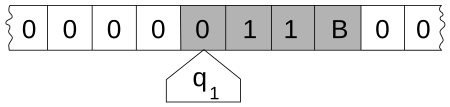
\includegraphics[width=6.5cm]{Turing_machine_2b.png}
	\begin{itemize}
		\item Modello matematico per descrivere funzioni calcolabili da un algoritmo
		\item \textbf{Funzioni calcolabili}: Funzioni parziali \( f : \mathbb{N} \rightarrow \mathbb{N} \) modellabili da una macchina di Turing
	\end{itemize}
\end{frame}

\section{Macchina di Turing quantistica}

\subsection{Configurazioni}

\begin{frame}{\subsecname}{}
	\centering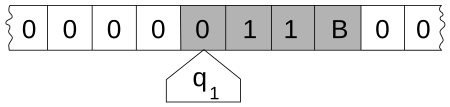
\includegraphics[width=6.5cm]{Turing_machine_2b.png}
	\begin{itemize}
		\item Una configurazione di una macchina di Turing è
		\[ \left \langle \alpha, q, \beta, i \right \rangle \in \Sigma^{*} \times \mathcal{Q} \times \Sigma^{*} \times \mathbb{Z} \]
		\item \textit{Q-configurazioni}: Elementi di \( \ell^{2}_{1} \left ( \Sigma^{*} \times \mathcal{Q} \times \Sigma^{*} \times \mathbb{Z} \times \mathbb{N} \right ) \)
		\item Definiamo \( \mathfrak{C}_M = \Sigma^{*} \times \mathcal{Q} \times \Sigma^{*} \times \mathbb{Z} \times \mathbb{N} \)
	\end{itemize}
\end{frame}

\subsection{Definizione}

\begin{frame}{\subsecname}{}
	\begin{itemize}
		\item Una pre-macchina di Turing quantistica è una tupla
		\[ M = \left \langle \Sigma \times \mathcal{Q} \times \mathcal{Q}_{s} \times \mathcal{Q}_{t} \times \delta_{0} \times q_{i} \times q_{f} \right \rangle \]
		\item Funzione \(\delta_{0}\)
		\[ \delta_{0} : \left ( \mathcal{Q} \backslash \mathcal{Q}_{t} \right ) \times \Sigma \rightarrow \ell^{2}_{1} \left ( \left ( \mathcal{Q} \backslash \mathcal{Q}_{s} \right ) \times \Sigma \times \mathbb{D} \right ) \]
		\item Una pre-macchina di Turing quantistica è una macchina di Turing quantistica se l'operatore di transizione \( U_{M} \) è unitario
	\end{itemize}
\end{frame}

\subsection{Operatore di transizione}

\begin{frame}{\subsecname}{}
	\begin{itemize}
		\item Definiamo \( U_{M} \) su ogni \(\left | C \right \rangle \) con \( C \in \mathfrak{C}_M \)
		\item Se \( C \in \mathfrak{C}^{0}_M \backslash \mathfrak{C}^{t}_M \)
		\[ U_{M} \left ( \left | C \right \rangle \right ) =
		\sum_{\left (p,v,d \right ) \in \left ( \mathcal{Q} \backslash \mathcal{Q}_{s} \right ) \times \Sigma \times \mathbb{D}}
		\delta_{0}(q, u)(p, v, d) \left | C_{p,v,d} \right \rangle \]
		\item Esiste un teorema che garantisce l'unitarietà se \(\delta_{0}\) rispetta certe condizioni
	\end{itemize}
\end{frame}

\section{Funzioni calcolabili quantistiche}

\subsection{PPD e computazioni}

\begin{frame}{\secname}{\subsecname}
	\begin{itemize}
		\item Una \textit{Partial Probability Distribution (PPD)} è una funzione \( \mathcal{P} : \mathbb{N} \rightarrow \mathbb{R}_{[0,1]} \) tale che \( \sum_{n \in \mathbb{N}} \mathcal{P} \left ( n \right ) \le 1 \)\par
		Una \textit{Probability Distribution (PD)} è una \textit{PPD} tale che \( \sum_{n \in \mathbb{N}} \mathcal{P} \left ( n \right ) = 1 \)
		\item A ogni \( \left | \phi \right \rangle \) si può associare una PPD \( \mathcal{P}_{\left | \phi \right \rangle} \)\par
		\( \mathcal{P}_{\left | \phi \right \rangle} \left ( n \right ) = \) probabilità di \( \left | \phi \right \rangle \) di collassare su una configurazione finale con \(n\) simboli \(1\) sul nastro 
	\end{itemize}
\end{frame}

\begin{frame}{\secname}{\subsecname}
	\begin{itemize}
		\item Una computazione \(K^{M}_{\left | \phi \right \rangle}\) è una sequenza \(\left | \phi_{i} \right \rangle\) tale che
		\begin{enumerate}
			\item \(\left | \phi_{0} \right \rangle = \left | \phi \right \rangle\) è una q-configurazione finale
			\item \(\left | \phi_{i} \right \rangle = U_{M}^{i}\left | \phi \right \rangle\)
		\end{enumerate}
		\item A ogni computazione si associa una sequenza di PPD \( \mathcal{P}_{\left | \phi_{i} \right \rangle} \)
		\item La sequenza \(\sum_{n \in \mathbb{N}} \mathcal{P}_{\left | \phi_{i} \right \rangle} \left ( n \right )\) è crescente
	\end{itemize}
\end{frame}

\subsection{Definizione}

\begin{frame}{\secname}{\subsecname}
	\begin{itemize}
		\item Prendiamo in considerazione funzioni di forma \( f : \ell^{2}_{1} \left ( \mathbb{N} \right ) \rightarrow PPD \)
		\item \( \mathcal{P} = \lim_{n \to \infty} \mathcal{P}_{\left | \phi_{i} \right \rangle} \) è l'\textit{output calcolato} di M
		\item Scegliamo una codifica da \( \ell^{2}_{1} \left ( \mathbb{N} \right ) \) a \( \ell^{2}_{1} \left ( \mathfrak{C}^{init}_M \right ) \)
		\item \textbf{Funzioni calcolabili quantistiche}: Funzioni \( f : \ell^{2}_{1} \left ( \mathbb{N} \right ) \rightarrow PPD \) rappresentabili da una Macchina di Turing quantistica
	\end{itemize}
\end{frame}

\subsection{Categorie di terminazione}

\begin{frame}{\subsecname}{}
	Una data computazione può
	\begin{enumerate}
		\item Produrre una \textit{PD} in un numero di passi finito
		\item Non produrre una \textit{PD} in un numero di passi finito, ma avere una \textit{PD} come \textit{PPD} limite
		\item Non avere una \textit{PD} come \textit{PPD} limite
	\end{enumerate}
\end{frame}

\section{Conclusione}

\begin{frame}{\secname}{}
	\begin{itemize}
		\item
	\end{itemize}
\end{frame}

\end{document}